\section*{Figure captions}
\begin{figure}[H]
\begin{center}
%\scalebox{1.5}{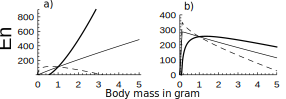
\includegraphics{Fig1}}
\caption{
	No warm-up. Resource is limiting
	Daily net energy gain  $E_n$ as function body mass $z$ for different value of foraging exponent $b_3 = 0.5,0.8, 1.25$ , dashed,think, thick lines respectively.
	The upper panels depict different resource availability at $15 ^{\circ} \rm{C}$. 
	Low resource = 2.5, intermediate resource= 20, unlimited resource means an individual can collect at 50 times its body mass, $b_2 = 0.75, a_2 = 20$. 
	The lower panels depict the influence of temperature when resources are unlimited and high cost of foraging $a_2 = 40, b_2  = 1.25$.
	Low, mild, and high temperature =$5, 15, 25 ^{\circ} \rm{C}$.
	Fixed parameter values: $b_1 = 0.75, \varepsilon = 16$.
}
\label{fig1}
\end{center}
\end{figure}
\vspace{-1.5cm}
%
\begin{figure}[H]
\begin{center}
%\scalebox{1.5}{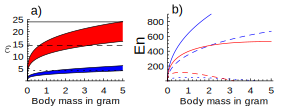
\includegraphics{Fig2}}
\caption{
	No warm-up. Time is limiting. foraging time = 0.5 hour.
	a) Daily net energy gain  $E_n$ as function body mass $z$ for different value of foraging exponent $b_3 = 0.5,0.8, 1.25$ , dashed,think, thick lines respectively  at $15 ^{\circ} \rm{C}$.
	b)  $E_n$ is maximized at intermediate value of $z$  when shaded regions and resource quality $\varepsilon$ intersect (i.e., \cref{C1} is satisfied).
	Warm (35 $^{\circ} \rm{C}$) and cold (15 $^{\circ} \rm{C}$) environmental temperatures are denoted by red and cyan, respectively.
	The upper (lower) limit of the shade region is $\widetilde{dE_n}$ ($\widetilde{E_n}$).  
	c) Various shapes of $E_n$ based on b).
	In b) and c), $\varepsilon = 13, 60, 100$ dashed, thin, and thick, respectively.
	Fixed parameter values: $b_1 = b_2 = 0.75, a_2 = 5 a_1, $.
}
\label{fig2}
\end{center}
\end{figure}
\vspace{-1.5cm}
%
\begin{figure}[H]
\begin{center}
%\scalebox{1.5}{\includegraphics{Fig3}}
\caption{
	Lowest temperature required for the completion of warm-up as a function of body mass.
	The individual is given a maximum of 6 hours to complete warm-up.
	To focus on the effect of solar radiation, daily temperature is constant.
	Solar radiation increases linearly from 0 to 0.25 of maximum value for 6 hours. 
	a) conductance is low (0.1 default value), b) conductance is default, wind speed  = 0.1m/s, c) for endotherm $a_w = 1.25$. 
	
	Fixed parameter values: default conductance $K_1 = 1, r_3 = 0.5  $
}% Add parameter values later
\label{fig3}
\end{center}
\end{figure}
\vspace{-1.5cm}
%
\begin{figure}[H]
\begin{center}
%\scalebox{1.5}{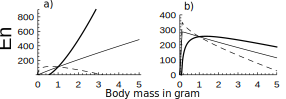
\includegraphics{Fig1}}
\caption{
	Duration of warm-up as a function of the timing of warm-up.
	Daily temperature varies from $15 ^{\circ}\rm{C}$ at sunrise  and peaks at $30 ^{\circ}\rm{C}$ at the middle of the afternoon.
	In a) and b), thickest, thick, thin, and dashed lines denote  $z = 10, 1, 0.1, 0.01$,  respectively.
	In c), thick, thin, and dashed gray lines denote high ($\times 10$), medium ($\times 1$), and low ($\times 0.1$) conductance between the rest-of-the-body and the thorax.
}% Add parameter values later
\label{fig4}
\end{center}
\end{figure}
\vspace{-1.5cm}
%
\begin{figure}[H]
\begin{center}
%\scalebox{1.5}{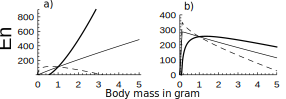
\includegraphics{Fig1}}
\caption{
	Shape of the niche as a function of temperature.
	Except in d),  temperature is constant during the day.
	a) The simplest case without warm-up, high resource availability (30 gram).
	b) Halving resource availability and without warm-up.
	c) Adding warm-up and  restoring resource availability to high.
	d) The most realistic scenario with warm-up, and variable temperature  which increases from 15 to 30 $^{\circ} \rm{C}$ from sunrise to mid afternoon.
Other parameters: $b_3 = 1, b_2 = b_1  = 0.75$, metabolic scope = 20, $a_w = 1.25$.
}% Add non trivial units later
\label{fig5}
\end{center}
\end{figure}
%